\documentclass[12pt,letterpaper]{article}
\usepackage[utf8]{inputenc}
\usepackage[margin=1in]{geometry}
\usepackage{booktabs}
\usepackage{tabu}
\usepackage{setspace}       % 1.5 spacing
\usepackage[labelfont=bf,skip=5pt,font=small]{caption}
\usepackage{subcaption}
\usepackage{graphicx}
\usepackage{fancyhdr}
\usepackage{listings}
\usepackage{lipsum}
\usepackage[onehalfspacing]
%\doublespacing
\setlength{\parskip}{1.5em}
\setlength{\parindent}{0em}


\begin{document}



\begin{center}
   \huge{\textbf{IOT CLOUD SMART GARBAGE MONITORING SYSTEM}}\\[8pt]
\end{center}

\rule{\textwidth}{0.5pt}
\begin{center}
    \large{\textit{Submitted in partial fulfilment of the requirements for the degree of}}\\
    \vspace{0.1 in}
    \large{\textbf{Masters of Technology}\\}
    \large{\textbf{In}\\}
    \large{\textbf{Computer Science and Engineering}}
\end{center}
\begin{center}
    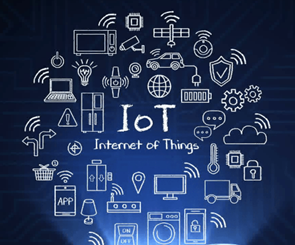
\includegraphics[height=3cm,width=3cm]{image.png}\\
    \vspace{0.1 in}
    \Large{\textbf{Submitted by}}\\
    \vspace{0.1 in}
    \large{Vudatha Venkata Narendra}\\
    \large{224101060}\\
    \vspace{0.2 in}
    \Large{\textbf{Under the guidance of}}\\
    \vspace{0.1 in}
    \large{\textbf{Dr. Manas Khatua}}\\
    \large{Asst. Professor}\\
    \large{Department of Computer Science and Engineering}\\
    \large{IIT Guwahati}\\
    \vspace{0.2 in}
    
\includegraphics[height=3cm,width=3cm]{IIT_Guwahati_Logo.svg.png}\\
    \small{September 2022}\\
\end{center}

\newpage
\begin{center}
    \large{\textbf{DECLARATION}}
\end{center}
I hereby declare that the thesis entitled \textbf{“IoT CLOUD SMART GARBAGE MONITORING SYSTEM”} submitted by Venkata Narendra Vudatha for the award of the degree of Bachelor of Technology in Programme to IIT Guwahati is a record of bonafide work carried out by Venkata Narendra Vudatha under the supervision of \textbf{Dr. Manas Khatua}. I further declare that the work reported in this thesis has not been 
submitted and will not be submitted, either in part or in full, for the award of any other degree or diploma in this institute or any other institute or university. \\
\begin{flushleft}
Place: Guwahati\\
Date: September 2022 \\
\end{flushleft}
\begin{flushright}
Signature of the Candidate \\
Venkata Narendra Vudatha\\
\end{flushright}



\newpage
\begin{center}
    \large{\textbf{List of Abbrevations}}\\
    \vspace{0.2 in}
    \begin{tabular}{ |p{3cm}|p{6cm}|  }
    \hline
    Short & Abbrevated\\
    \hline
     NodeMCU   & Node Micro controller unit\\
     IoT   & Internet of Things\\
     GND   & Ground\\
     VCC   & Voltage common collector\\
     RISC   & Reduced Instruction Set Computer\\
     GPIO   & General-Purpose Input/Output\\
     RTOS   & Real-Time Operating System\\
     LCD   & Liquid Crystal Display\\
     LED   & Light Emitting Diode\\
     ADC   & Analog to Digital Converter\\
     USB   & Universal Serial Bus\\
     Wi-Fi   & Wireless Fidelity\\
     M Hz   & Megahertz\\
     PC   & Personal Computer\\
     IDE   & Integrated Development Environment\\
     \hline
    \end{tabular}
\end{center}


\newpage

\tableofcontents
\newpage

\typeout{}
\include{Main Obkective}
\cleardoublepage 
\typeout{}
\include{Main Obkective}
\cleardoublepage

\section{Introduction}
IoT (Internet of Things) is first invented in 1999, by Kevin Ashton. The simple meaning of IoT can be defined as a connection of sensors which collect data and send to the cloud which in turn computes it and gives triggers to the actuators by using whom we act on the environment. It is being used in Industry purpose, Scientific purposes, and medical purposes mainly which have desired bands and there are many more purposes where we use IoT and its even becoming hard to find an area where IoT is not being used. Even though it is coined in 1999 it did not get that importance and usage then.

In the present world IoT (Internet of Things) are emerging, adapted and most hyped phenomenon in the current decade. This is because of the flexibility and the options it provides to the users to use in various domains is the main reason, since it can be used from the basic toilet monitoring system to the greatest applications like controlling and getting the whole details of a company like number of persons entering monitoring temperatures etc... and many more. Other staggering features that IoT provides are the scalability, security, adaptability, and cost effectiveness which are very much important while considering a real-world application.
\subsection{MAIN OBJECTIVE: }
The main objective of this project is to gain better knowledge about Internet of Things which is very much emerging in the recent decades and we can feel the its flow passing all over and to implement the learned knowledge on the “IoT CLOUD SMART GARBAGE MONITORING SYSTEM.” These days the popularity and the usage of Internet of Things has been increasing so rapidly, so making our own project using learning about Internet of Things is helpful in career perspective of a student. 

The objectives we are going to provide to the users using our project are: - 
\begin{itemize}
    \item Detecting dustbin level
    \item Displaying the garbage level in dustbin.
    \item Sending an email to the authority when the garbage level exceeds 80%.
    \item A website through which we can check the garbage level.
    \item Easy to understand interface.
    \item Less overhead and fast computation of level.
    \item A healthy environment (as the waste in their areas gets removed)
\end{itemize}

\subsection{MOTIVATION: }
In many places of India, the dustbins are not being cleaned even though it is filled with garbage, so the garbage is coming out this is happening due to lack of information to the authorities that a dustbin of a particular area is being filled with dust or else they may take much more time to check and get it fixed this is where the problem arises. This leads to various problems like increasing of bacteria and viruses along with the raise of mosquitos and some other insects. This may cause many insectivorous diseases to the nearby people. Moreover, it is not even good for global warming since this waste can contain any thing and combination of different types of wastes could lead to release of poisonous gasses and hence cause global warming.  This is not only the case for one area it should be resolved. For this we need a cost effective and easy to implement interface to handle. 
IoT helps in doing all this in an easy and simple way. We can implement all the required set up with the help of just a NodeMCU, an ultrasonic sensor, a bread board, and few jumper wires which is very much affordable for government since it does not cost much and we can implement this and get the desired outputs. These are all lower power consuming devices so there will not be any necessities like frequent change in batteries or something else we can once setup and can forget about them for next 5-10 years.




\newpage
\section{DESIGN ATTRIBUTES AND DESIGN}
In this part I am going to explain how I made my connections in order to make my circuit work and what are all the attributes that are being used here.
\subsection{CONFIGURATION DIAGRAM:}
\begin{figure}[htp]
        \centering
        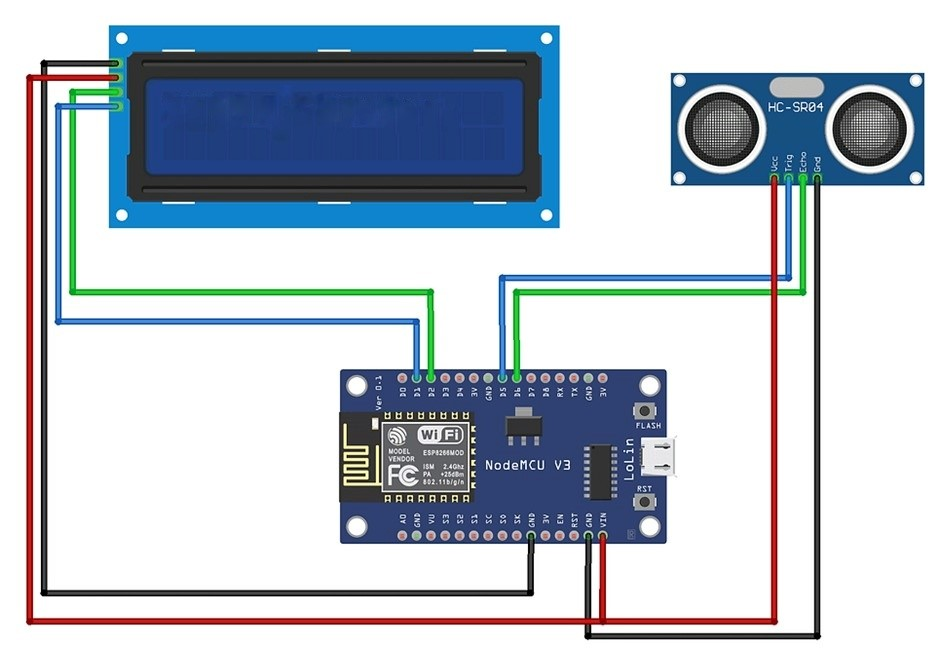
\includegraphics[width=\textwidth]{circuit diagram.jpg}
        \caption{circuit diagram }
        \label{fig:image3}
    \end{figure}

\subsection{COMPONENTS:}
\begin{enumerate}
    
    \item \textbf{HC-SR04 sensor} : It is an ultrasonic sensor, also known as an ultrasonic transducer that is based on a transmitter and receiver and mainly used to determine the distance from the target object. The amount of time it takes to send and receive waves will determine how far the object is placed from the sensor. It mainly depends on the sound waves working on “non-contact” technology. The required distance of the target object is measured without any damage, giving you accurate and precise details. This sensor comes with a range between 2cm to 400cm and is used in a wide range of applications including speed and direction measurement, wireless charging, humidifiers, medical ultrasonography, sonar, burglar alarms, and non-destructive testing.
    \begin{figure}[h!]
        \centering
        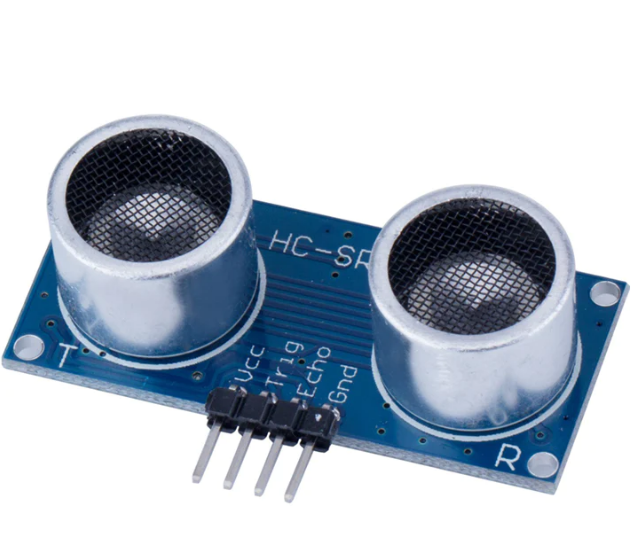
\includegraphics[height=5cm,width=7cm]{HC-SR04 sensor.png}
        \caption{HC-SR04 sensor}
        \label{fig:image3}
    \end{figure}
    
    \begin{figure}[h!]
        \centering
        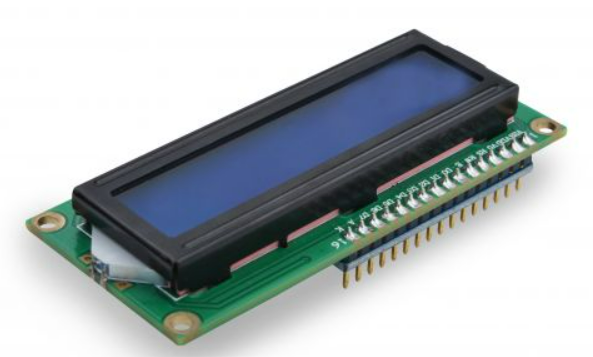
\includegraphics[height=7cm,width=10cm]{16x2.I2c LCD display.png}
        \caption{16x2.I2c- LCD display}
        \label{fig:image3}
    \end{figure}
    \item \textbf{16x2.I2c- LCD display :}  It is an electronic device that is used to display data and the message is known as LCD 16×2.  it includes 16 Columns and 2 Rows so it can display 32 characters (16×2=32) in total and every character will be made with 5×8 (40) Pixel Dots. So, the total pixels within this LCD can be calculated as 32 x 40 otherwise 1280 pixels. 16 X2 displays mostly depend on multi-segment LEDs. The basic working principle of LCD is passing the light from layer to layer through modules. These modules will vibrate and line up their position on 90o that permits the polarized sheet to allow the light to pass through it. These molecules are accountable for viewing the data on every pixel. Every pixel utilizes the method of absorbing light to illustrate the digit. To display the value, the position of molecules must be changed to the angle of light. So, this light deflection will make the human eye notice the data that will be the ingredient wherever the light gets absorbed.
    
    \begin{figure}[h!]
        \centering
        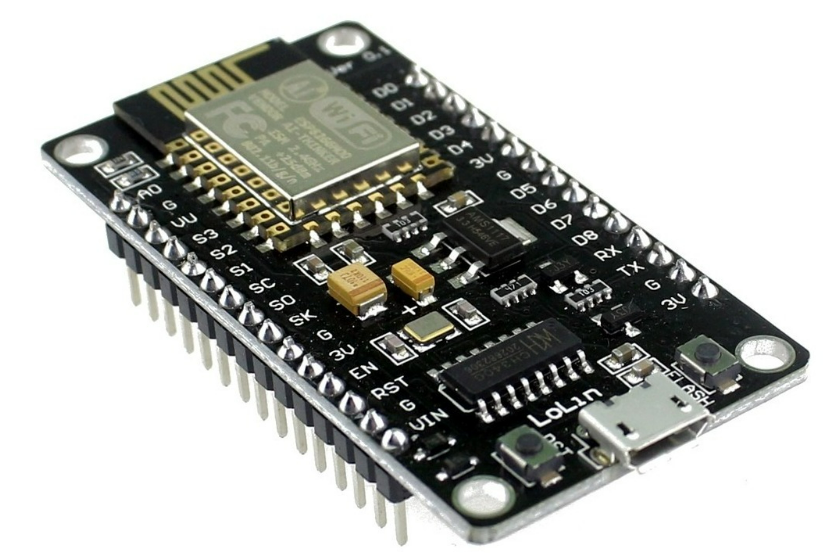
\includegraphics[height=7cm,width=10cm]{ESP8266 I2e- NodeMCU.png}
        \caption{ESP8266 12e- NodeMCU}
        \label{fig:image3}
    \end{figure}
    \item \textbf{ESP8266 12e- NodeMCU :}ESP8266 NodeMCU is a popular and widely used development board based on the ESP-12E Wi-Fi Module that combines elements of easy programming with Arduino IDE (C or C++) and Wi-Fi capability. Through the build-in programmer and CH340G USB-to-Serial chip, flashing the ESP8266 and serial output on a PC, development and prototyping projects are done with ease. Just like Arduino boards, the ESP8266 NodeMCU has GPIO pins, voltage regulator, ADC, Micro-USB port (for flashing and serial output) – all on one board. On top of that the ESP8266 NodeMCU has a full Wi-Fi that takes care of the Wi-Fi communication to a server or client. ESP8266 consists of a Tensilica L106 32-bit micro controller unit (MCU) and a Wi-Fi transceiver. It has 11 GPIO pins* (General Purpose Input/Output pins), and an analog input as well. The ESP8266EX integrates a Tensilica L106 32-bit RISC processor, which achieves extra-low power consumption and reaches a maximum clock speed of 160 MHz The Real-Time Operating System (RTOS) and Wi-Fi stack allow 80 percentage of the processing power to be available for user application programming and development.
    
    \begin{figure}[h!]
        \centering
        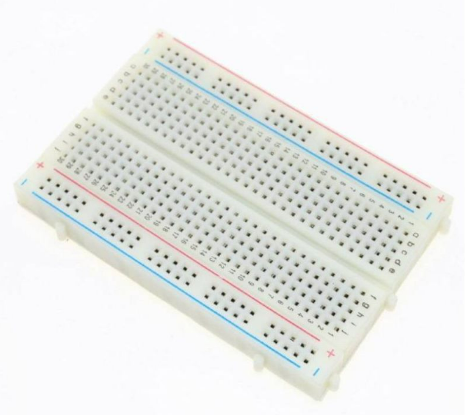
\includegraphics[height=7cm,width=10cm]{bread board.png}
        \caption{Bread board}
        \label{fig:image3}
    \end{figure}
    \item \textbf{Bread board: }A Breadboard is simply a board for prototyping or building circuits on. It allows you to place components and connections on the board to make circuits without soldering. The holes in the breadboard take care of your connections by physically holding onto parts or wires where you put them and electrically connecting them inside the board. The ease of use and speed are great for learning and quick prototyping of simple circuits. More complex circuits and high frequency circuits are less suited to breadboarding. The two larger pieces of wire down each side are typically used to connect a power source to the board. They are usually referred to as power rails. The other smaller pieces of wire running perpendicular all the way across the board is used for components in your circuit.
    
    \begin{figure}[h!]
        \centering
        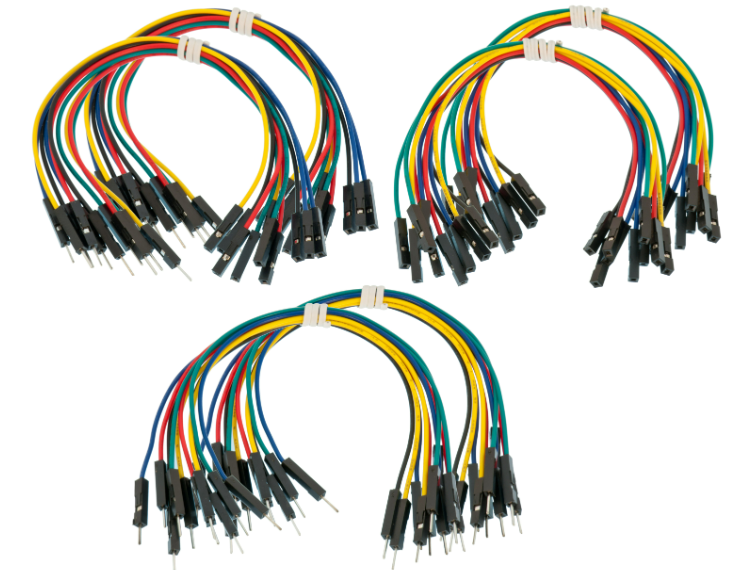
\includegraphics[height=7cm,width=10cm]{Jumper wires.png}
        \caption{Jumper wires}
        \label{fig:image3}
    \end{figure}
    \item \textbf{Jumper wires:}A jump wire (also known as jumper, jumper wire, DuPont wire) is an electrical wire, or group of them in a cable, with a connector or pin at each end (or sometimes without them – simply "tinned"), which is normally used to interconnect the components of a breadboard or other prototype or test circuit, internally or with other equipment or components, without soldering. Jumper wires typically vary in colour and size depending on what they are being used for. In breadboards, jump wires are used to establish connections between the central micro controller and other devices such as buttons and sensors. If possible, the jumper wire should always be placed on the component side of a circuit board during assembly. The wires should also be routed in an X-Y manner, avoiding any bends. Jump wires should never be raised more than 1/8 of an inch above the surface of the circuit board.
    
\end{enumerate}


\subsection{IMPLEMENTED ATTRIBUTES:}
The attributes that are being used in my project are:
\begin{enumerate}
    \item \textbf{Sensor:} I used Ultrasonic sensor for getting my input i.e., height of garbage.
    \item \textbf{Actuator:} Cayenne platform is used as actuator which sends SMS or email to the respected authority when the alert is triggered.
    \item \textbf{Cloud:} I send the data to Cayenne platform which acts as a cloud and displays data in a guage and a cylinder which makes easy for the users to understand.
    \item \textbf{Node MCU :} This is the development board that I used in my project which works similar to Arduino board.
    \item \textbf{ESP8266 :}This is used as a Wi-Fi module to communicate with server or client. To send data to the cloud a Wi-Fi module is necessary.
    \item \textbf{Computation:} Node MCU consists of a Tensila L106 32-bit micro controller unit which is a RISC processor with low power consumption and reaches a maximum clock speed of 160M Hz .Cayenne platform is used to compute the data and decide whether to give command to actuator
    \item \textbf{Alert Mechanism :} The alert mechanism that I have used in my project is to send a notification to the respected authority when the garbage level of the dustbin reaches more than 80 percent.
\end{enumerate}


\newpage
\section{PROJECT DEMONSTRATION}
In this part I am going to explain about the source code and the implementation.
\subsection{CODES:}
\begin{lstlisting}
#include <ESP8266WiFi.h>
#include <HCSR04.h>
#include <LiquidCrystal_I2C.h>
#include <CayenneMQTTESP8266.h>

LiquidCrystal_I2C lcd(0x27,16,2);

//Giving the details of my wifi to connect.
char ssid[] = "Bottle Cap"; // your SSID
char password[]="vvnarendra_10";  // your password

// Cayenne authentication info. This should be obtained from the Cayenne Dashboard.
char username[] = "13504de0-2b63-11ed-baf6-35fab7fd0ac8";
char mqtt_password[] = "eb10ac31d0a629e8424435436bd2ca42a39a03c5";
char client_id[] = "044ae3e0-3c3a-11ed-bf0a-bb4ba43bd3f6";

#define MAX_HEIGHT 20 // your bin height
int Percentage;

UltraSonicDistanceSensor distanceSensor(D5,D6);  //D1 trig, D2=ech

void setup(void)
{
  Serial.begin(115200);
   Cayenne.begin(username,mqtt_password,client_id,ssid,password);// starting cayenne 
  delay(1000);
  lcd.init();                      
  // initialize the lcd 
  // Print a message to the LCD.
  lcd.backlight();
}

void loop()
{
     Cayenne.loop();
    float actualCM=1*distanceSensor.measureDistanceCm();    
   // Serial.println(actualCM); 
Percentage=(MAX_HEIGHT-actualCM)/(MAX_HEIGHT-5)*100  ;
    Serial.println(Percentage);
    lcd.clear();
    lcd.setCursor(0,0);
    lcd.print(" IOT Smart BIN  ");
    lcd.setCursor(0,1);
    lcd.print("Waste Fill:");
    lcd.setCursor(11,1);
    lcd.print(Percentage);
    lcd.setCursor(13,1);
    lcd.print(" % ");
    delay(1000);
    Cayenne.virtualWrite(1, Percentage);
    if(Percentage>=100)
      { 
        lcd.setCursor(11,1);
        lcd.print("FULL  ");             
        delay(1000);
      }      
   }

\end{lstlisting}

\subsection{IMPLEMENTATION:}
\begin{enumerate}
    \item Circuit connections: Starting with the ultrasonic sensor it has 4 pins which are connected to NodeMCU in this way:\\
    \begin{tabular}{ |p{3cm}|p{3cm}|  }
    \hline
    Pin in sensor & Connection in NodeMCU\\
    \hline
     VCC   & Vin\\
     Trig  & D5\\
     Echo  & D6\\
     Grd   & GND\\
     \hline
    \end{tabular}
    \vspace{0.1 in}\\
    Connections from LCD to NodeMCU\\ 
    \vspace{0.1 in}
    \begin{tabular}{ |p{3cm}|p{3cm}|  }
    \hline
    Pin in LCD & Connection in NodeMCU\\
    \hline
     GND   & GND\\
     Vcc   & Vin\\
     SDA   & D2\\
     SCL   & D1\\
     \hline
    \end{tabular}
    \item Cayenne setup: This acts like the cloud for my project. To make this work we need to :
    \begin{itemize}
        \item Go to my.devices.com
        \item Create a cayenne account
        \item Select ESP8266 module.
        \item Copy client id, password and user id and paste in code.
        \item Name this module with some named (I named Generic ESP8266).
        \item Click on Add new -> select device/widget ->select gauge and then do remaining settings like analog and max to 100 and min to 0.
        \item Similarly add a tank widget.
        \item Go to add trigger and set it to send message and email if the threshold in gauge is more than 80 percet. (Means we get a notification when the bin is filled with more than 80 percent of the garbage).
    \end{itemize}
    \item Node MCU code: First go to IDE and download the required libraries.\\
    Include the required libraries in the code (I included ESP8266WiFi, HCSR04, LiquidCrystal-I2C, CayenneMQTTESP8266).\\
    Define the height of dustbin in centimetres (I used 20). \\
    Initialize the LCD display.\\ 
    Give the details of the Wi-Fi (username and password).\\
    Give the Cayenne information (username, mqtt password, client id).\\
    Initialize percentage to integer.\\
    Start the serial monitor and Cayenne to get information.\\
    Initialize LCD and print on it.\\
    Distancesensor is the variable used to calculate the distance between from the pins D5 and D6.\\
    I get the actual height from the Distancesensor.\\
    I set to display percentage when the garbage filled percentage is less than 100 and show FULL if it is 100. \\
    I made this data send to Cayenne and then it will trigger if required.\\
\end{enumerate}

\subsection{SAMPLE OUTPUT}
    \begin{figure}[htp]
        \centering
        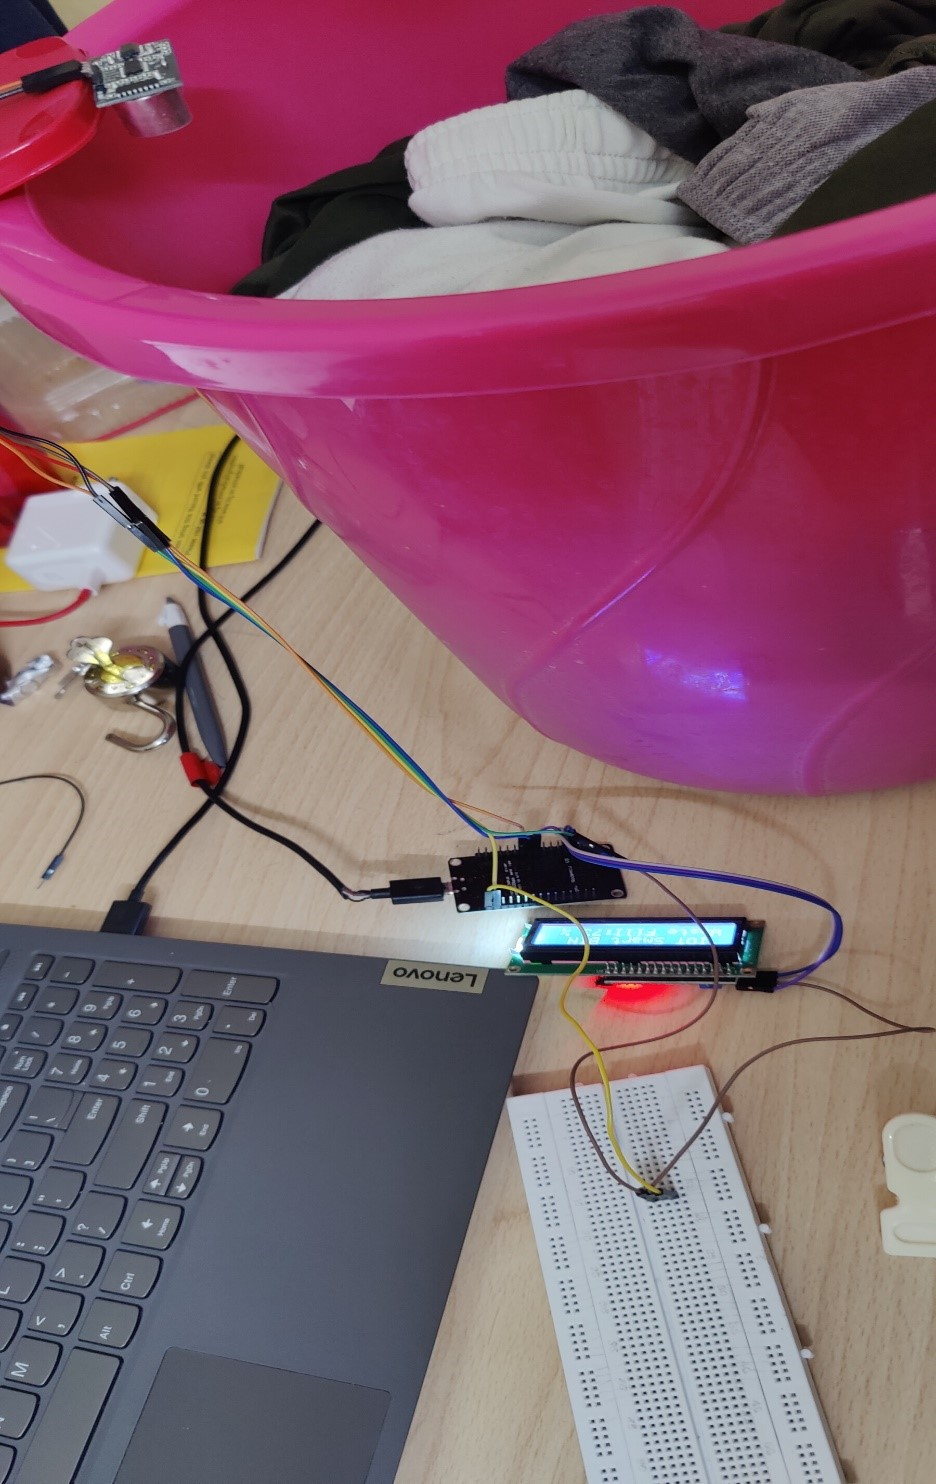
\includegraphics[height= 23cm, width=\textwidth]{original circuit diagram.jpg}
        \caption{Original circuit diagram which is connected}
        \label{fig:image3}
    \end{figure}
    \begin{figure}[htp]
        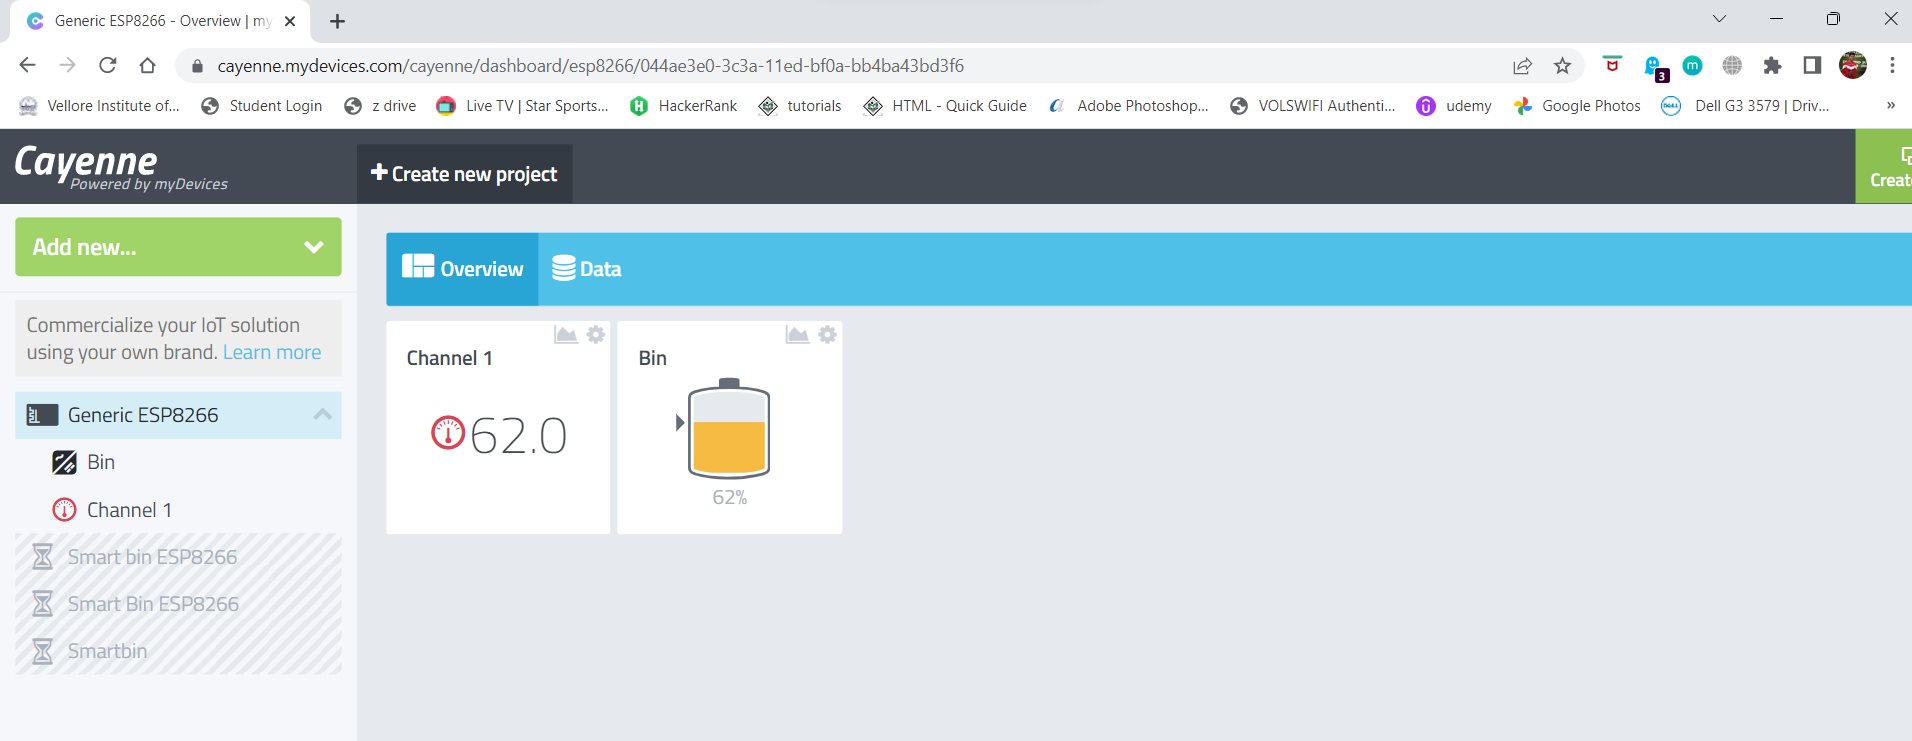
\includegraphics[width=\textwidth]{Cayenne platform op.png}
        \caption{Cayenne platform output}
        \label{figure: image4}
    %\end{figure}
    %\begin{figure}[htp]
        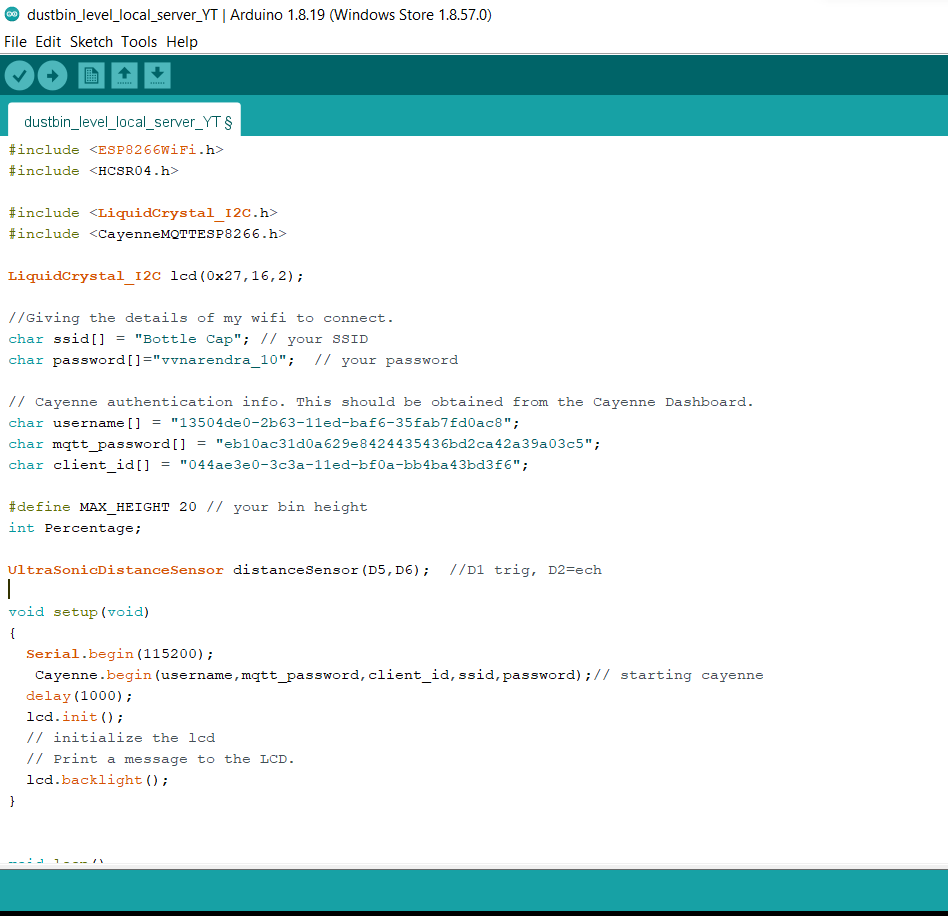
\includegraphics[width=\textwidth]{IDE Code 1st half.png}
        \caption{IDE Code 1st half}
        \label{figure: image4}
    \end{figure}
    \begin{figure}[htp]
        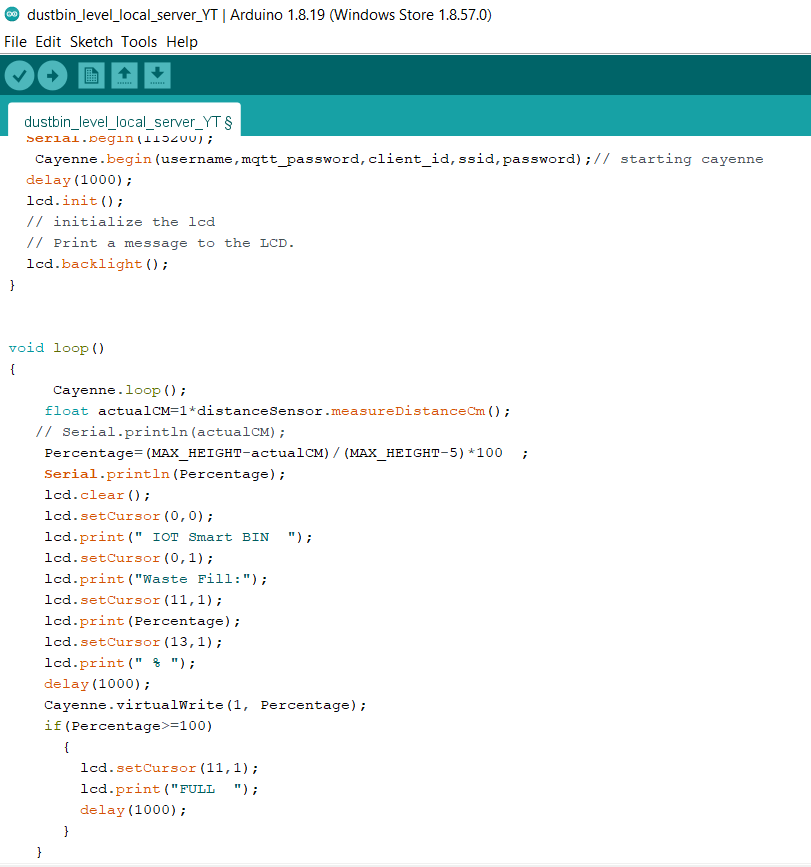
\includegraphics[width=\textwidth]{IDE Code 2nd half.png}
        \caption{IDE Code 2nd half}
        \label{figure: image4}
    \end{figure}
    \begin{figure}[htp]
        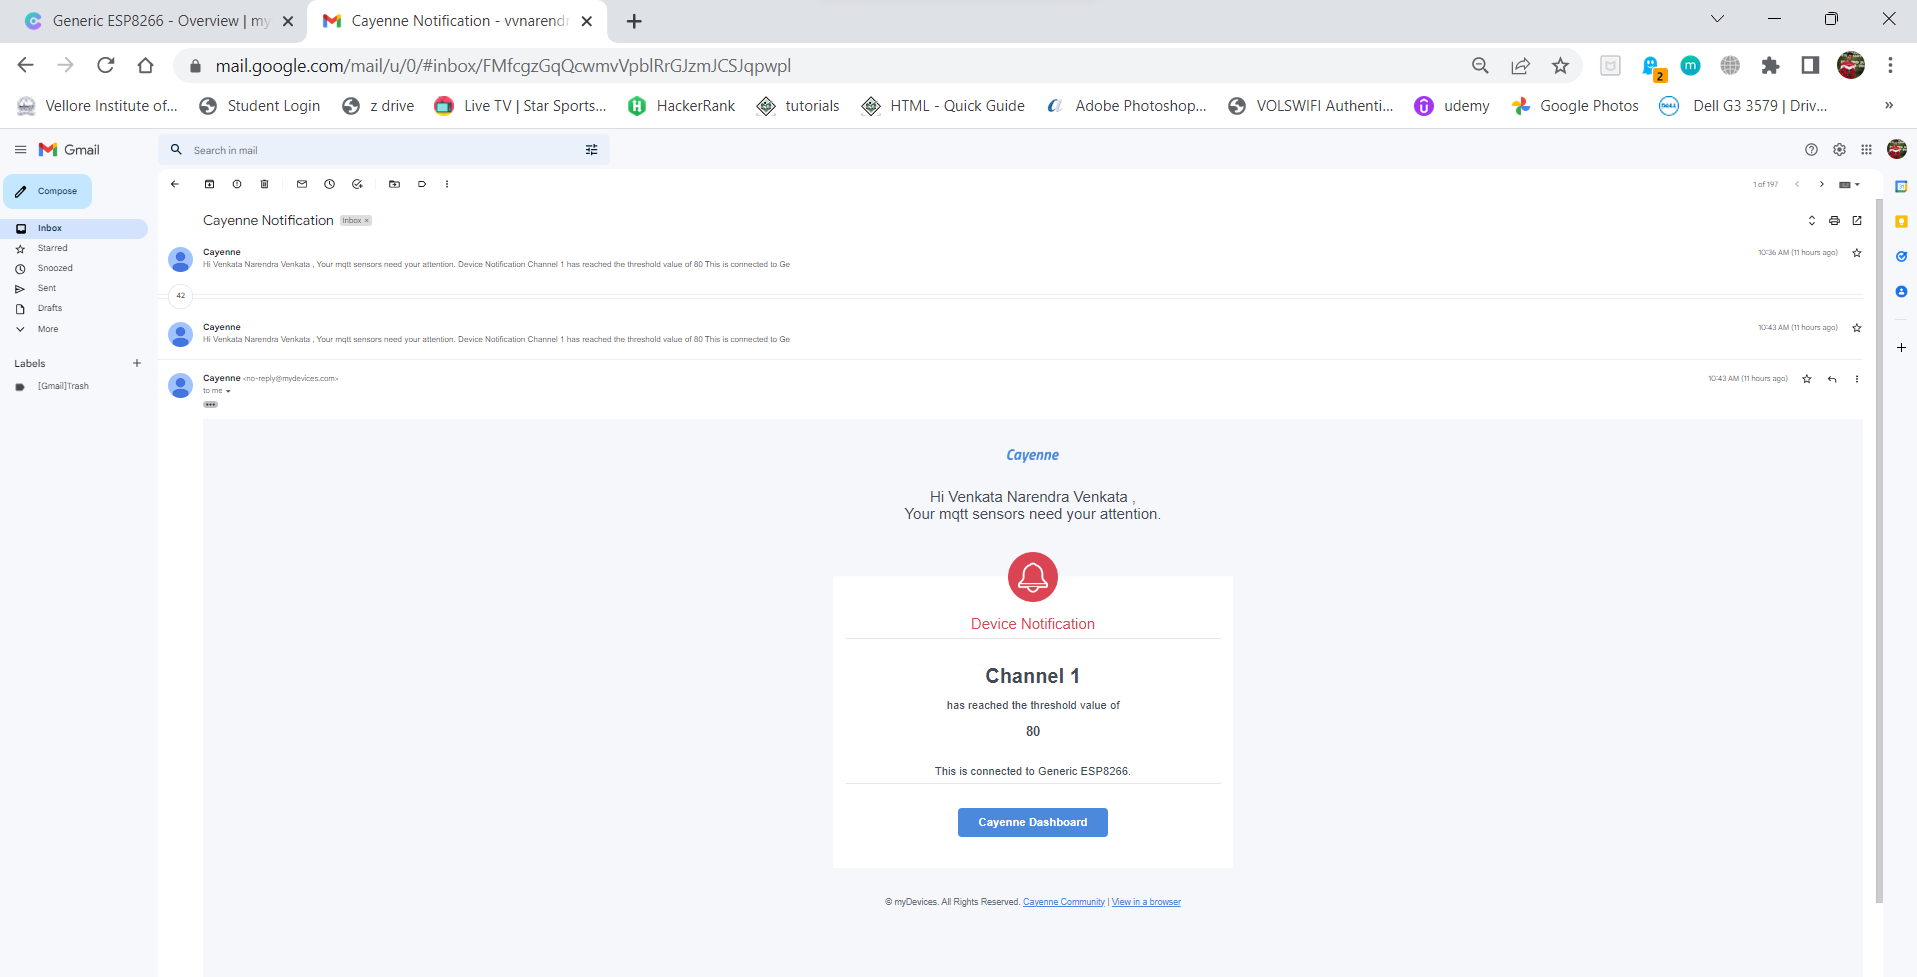
\includegraphics[width=\textwidth]{email notification Cayenne.png}
        \caption{Email notification by Cayenne}
        \label{figure: image4}
    \end{figure}
    \begin{figure}[htp]
        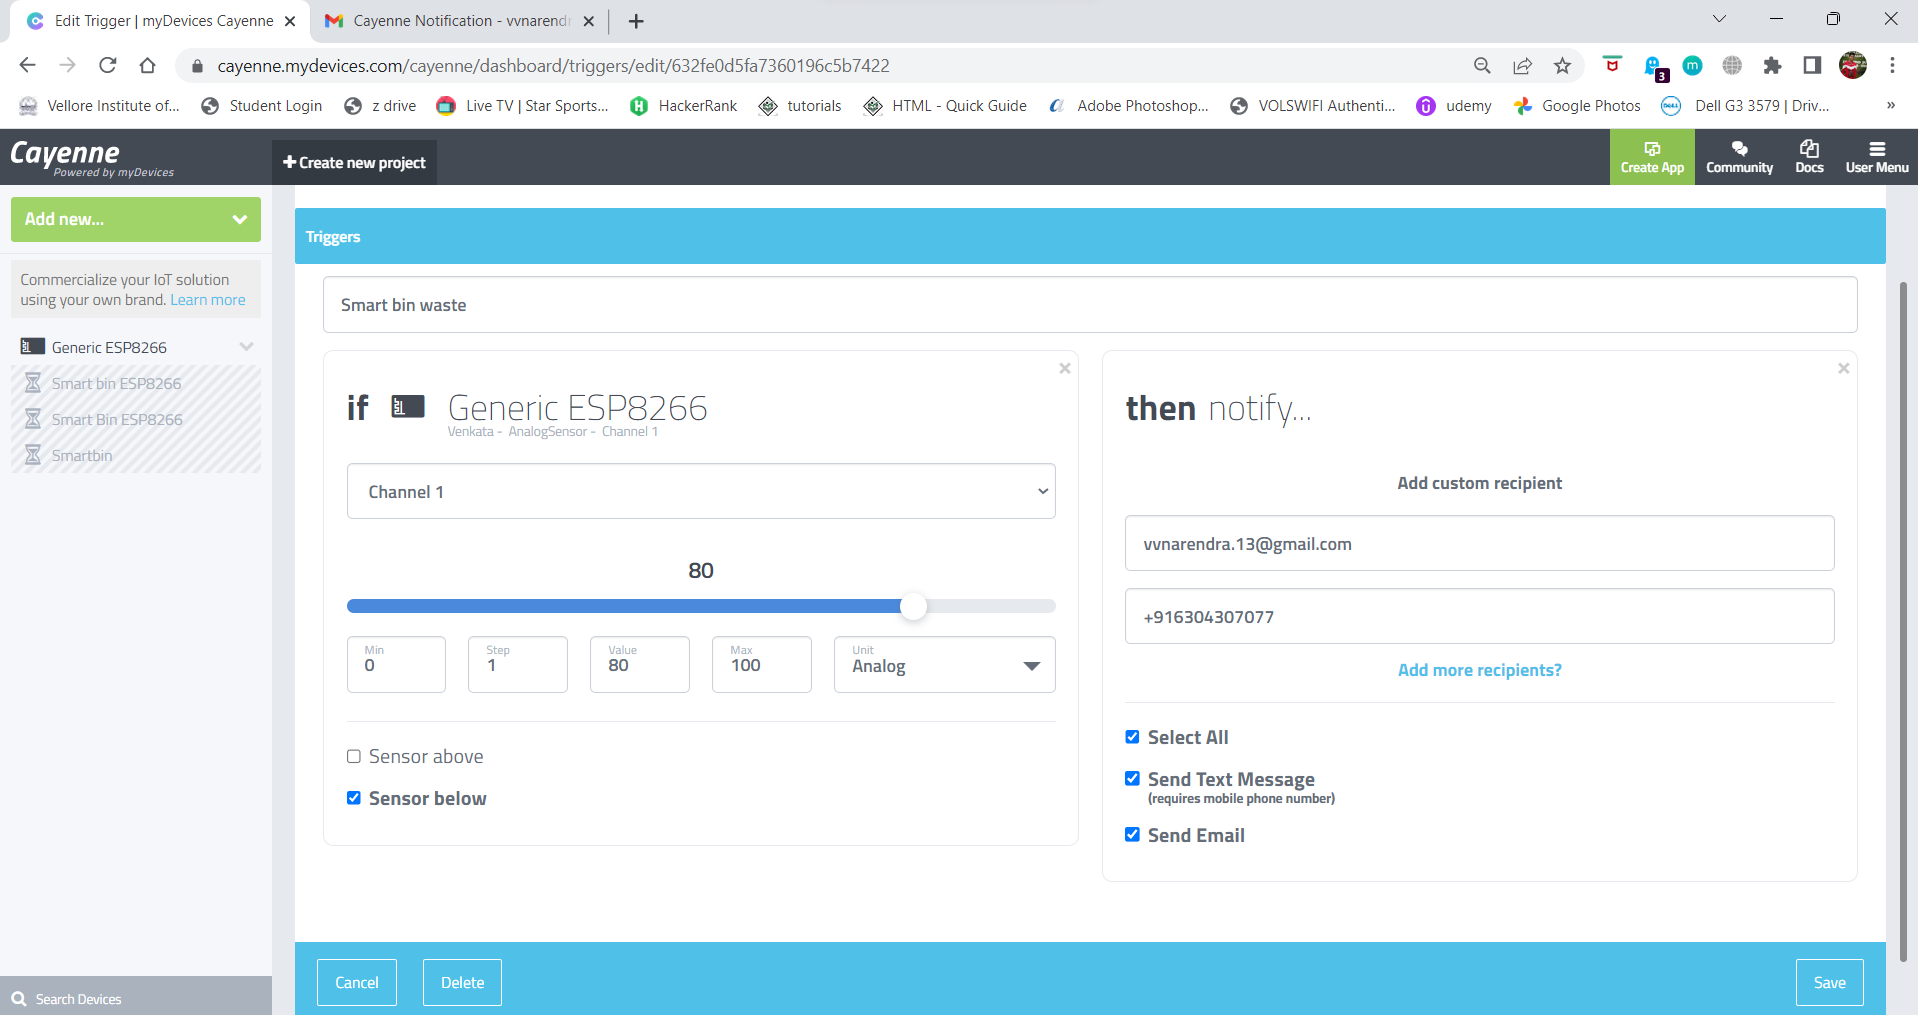
\includegraphics[width=\textwidth]{Cayenne Trigger.png}
        \caption{Cayenne trigger}
        \label{figure: image4}
    \end{figure}
    \begin{figure}[htp]
        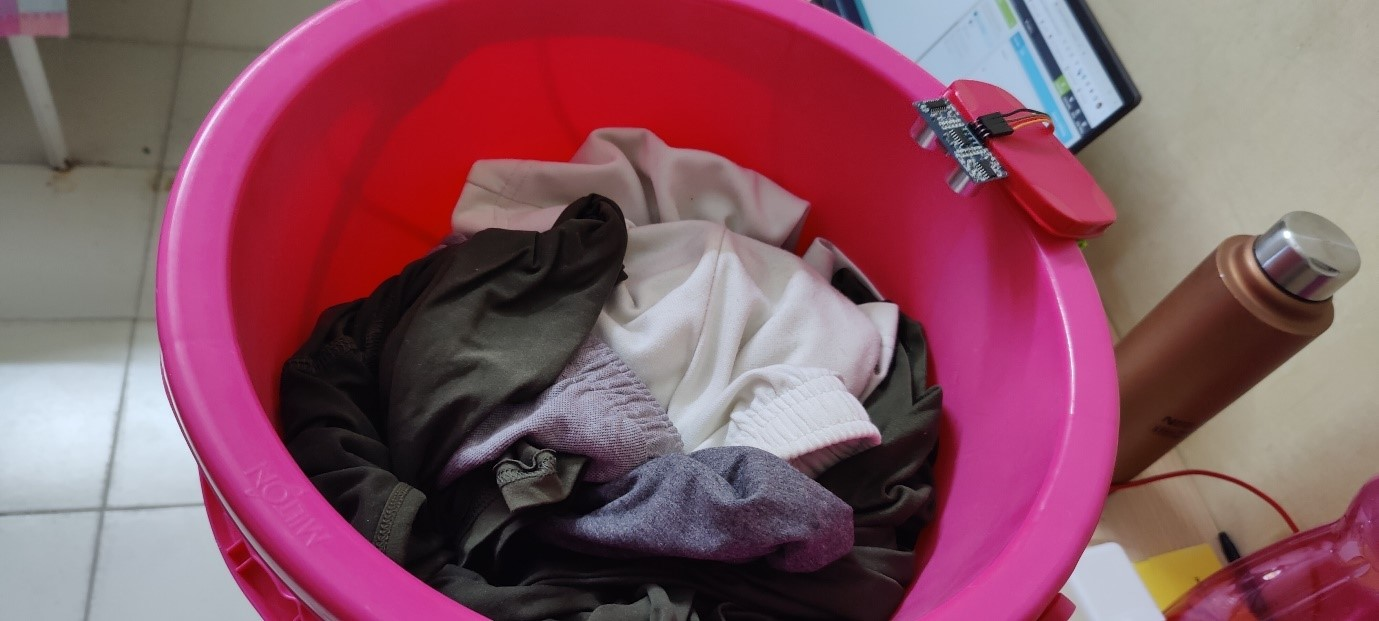
\includegraphics[width=\textwidth]{Bin filled with waste.jpg}
        \caption{Bin filled with garbage}
        \label{figure: image4}
    \end{figure}
    \begin{figure}[htp]
        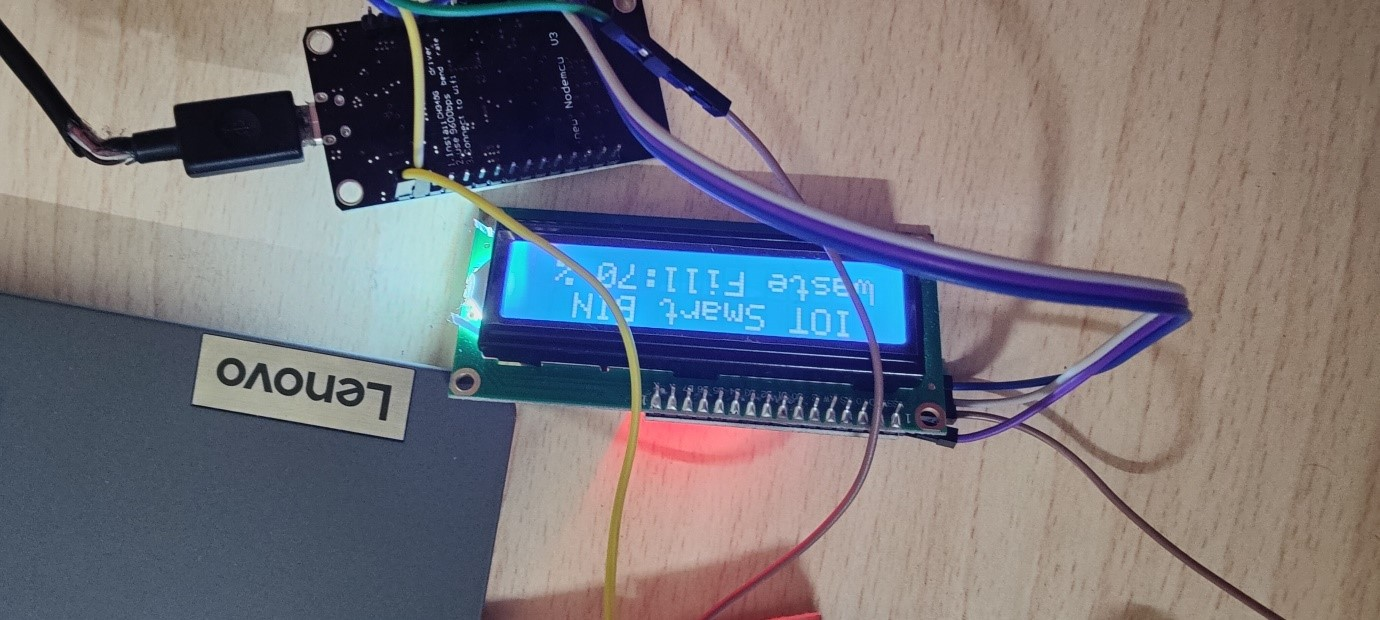
\includegraphics[width=\textwidth]{LCD dust level.jpg}
        \caption{LCD showing dust level in Bin}
        \label{figure: image4}
    \end{figure}

\newpage
\section{COST ANALYSIS}
The cost can be calculated in 2 ways one in the way of cost to buy the components and the other for the cost of deploying and making the circuit.
\begin{enumerate}
    \item The cost for buying the components is minimal because we just need few jumper wires where each will cost around 1 ½ rupees and the LCD display is not necessary when we are using this project to be implemented in real time and the ultrasonic sensor takes some 80 rupees whereas the NodeMCU is around 250 rupees. Summing up all these makes this an economical project. 
    \item When it comes to deployment cost, it does not take even a single rupee and the time to deploy is also less we just need to download all the required libraries into the IDE and then we can send them to any number of NodeMCU and implement is no time.
\end{enumerate}

\newpage
\section{User Manual}
\begin{enumerate}
\item Place the ultrasonic sensor at the edge of dustbin such that it can see the complete level of dustbin.
\item Make the connections in such a way as shown in figure and send code to NodeMCU.
\item Throw garbage in the dustbin.
\item The percentage level with how much garbage the bin is filled with is displayed on the cayenne dashboard in form of a gauge and tank.
\item Keep adding more dust to the bin now if the level of the waste in it increases to more than 80 percentage then the alert is triggered from Cayenne platform.
\item Now the concerned or respected authority will get a notification in form of a mail or a text message and they can clean it.
\end{enumerate}
%\printbibliography

\newpage
\section{SUMMARY}
\subsection{SUMMARY: }
The main objective of this project is that it can be used in real-time and can be helpful in reducing the spread of insectivorous diseases which is very important. The implementation starts with the connections with NodeMCU and the sensor along with the LCD display. So, after making the connection I wrote the code such that it will calculate the height of the garbage and all these information is send too the Cayenne platform in which it will send a notification to the authorities if the bin is filled with more than 80 percent of waste. 
Meanwhile the percentage of garbage is being calculated from the sensor information and is being displayed on the LCD display screen. When it comes to the future enhancements, I have ideas to implement like: segregating the wet waste and dry waste based on the waste a person puts in it and then use different sensors to finds different levels of garbage value filled. And the idea is like making the garbage flat and then calculating distance because if the waste is tilted then we end up with incorrect values sensing at other end this could give the authority that garbage value is more than 80 percent but in reality, it would be around 60 percent so this improvement is helpful.

\subsection{VIDEO LINK: }
\textbf{Video link :}https://1drv.ms/v/s!AnY29BjVd5tE1H8kdB8fWmVrvRPw

\end{document}